% Created by tikzDevice version 0.12.3.1 on 2022-10-11 18:23:57
% !TEX encoding = UTF-8 Unicode
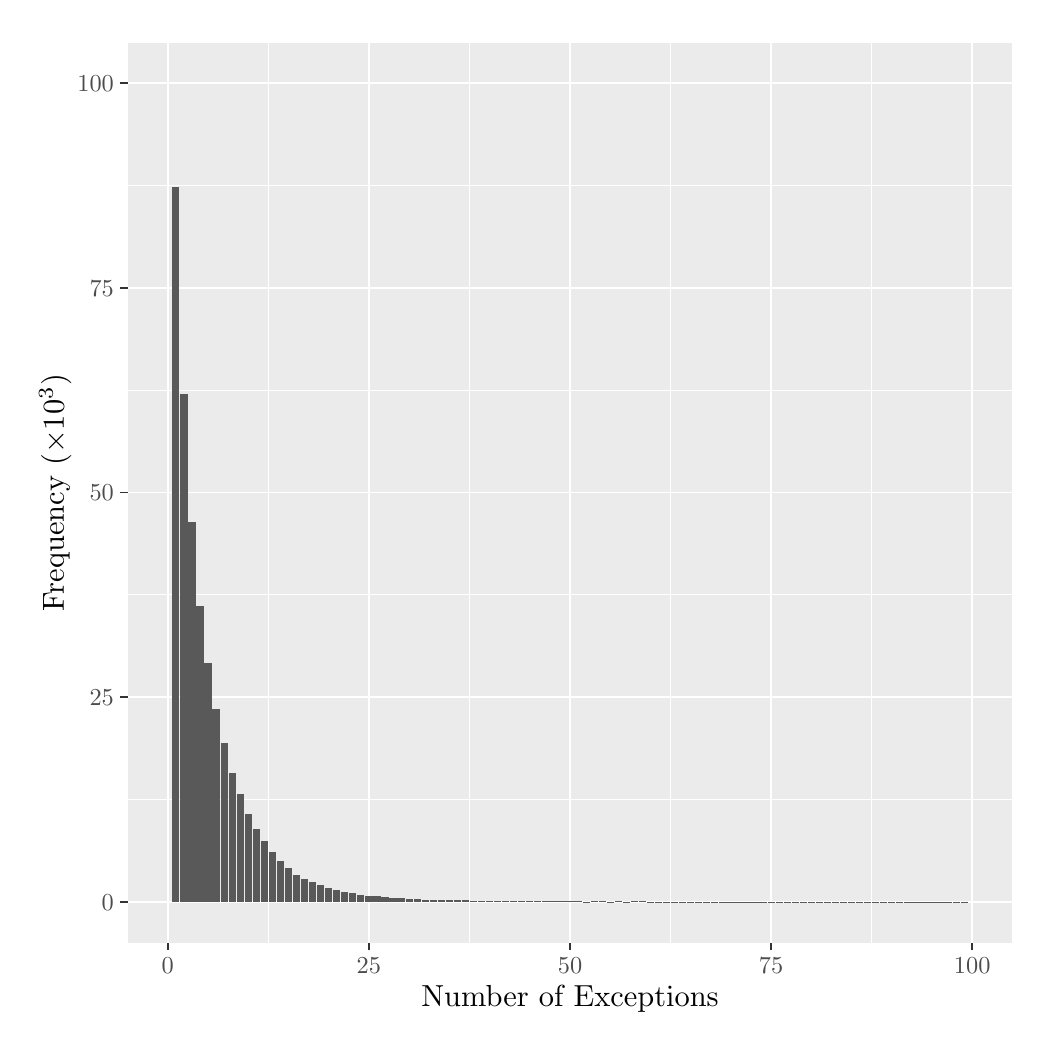
\begin{tikzpicture}[x=1pt,y=1pt]
\definecolor{fillColor}{RGB}{255,255,255}
\path[use as bounding box,fill=fillColor,fill opacity=0.00] (0,0) rectangle (361.35,361.35);
\begin{scope}
\path[clip] (  0.00,  0.00) rectangle (361.35,361.35);
\definecolor{drawColor}{RGB}{255,255,255}
\definecolor{fillColor}{RGB}{255,255,255}

\path[draw=drawColor,line width= 0.6pt,line join=round,line cap=round,fill=fillColor] (  0.00,  0.00) rectangle (361.35,361.35);
\end{scope}
\begin{scope}
\path[clip] ( 36.11, 30.69) rectangle (355.85,355.85);
\definecolor{fillColor}{gray}{0.92}

\path[fill=fillColor] ( 36.11, 30.69) rectangle (355.85,355.85);
\definecolor{drawColor}{RGB}{255,255,255}

\path[draw=drawColor,line width= 0.3pt,line join=round] ( 36.11, 82.45) --
	(355.85, 82.45);

\path[draw=drawColor,line width= 0.3pt,line join=round] ( 36.11,156.42) --
	(355.85,156.42);

\path[draw=drawColor,line width= 0.3pt,line join=round] ( 36.11,230.38) --
	(355.85,230.38);

\path[draw=drawColor,line width= 0.3pt,line join=round] ( 36.11,304.35) --
	(355.85,304.35);

\path[draw=drawColor,line width= 0.3pt,line join=round] ( 86.98, 30.69) --
	( 86.98,355.85);

\path[draw=drawColor,line width= 0.3pt,line join=round] (159.65, 30.69) --
	(159.65,355.85);

\path[draw=drawColor,line width= 0.3pt,line join=round] (232.31, 30.69) --
	(232.31,355.85);

\path[draw=drawColor,line width= 0.3pt,line join=round] (304.98, 30.69) --
	(304.98,355.85);

\path[draw=drawColor,line width= 0.6pt,line join=round] ( 36.11, 45.47) --
	(355.85, 45.47);

\path[draw=drawColor,line width= 0.6pt,line join=round] ( 36.11,119.43) --
	(355.85,119.43);

\path[draw=drawColor,line width= 0.6pt,line join=round] ( 36.11,193.40) --
	(355.85,193.40);

\path[draw=drawColor,line width= 0.6pt,line join=round] ( 36.11,267.37) --
	(355.85,267.37);

\path[draw=drawColor,line width= 0.6pt,line join=round] ( 36.11,341.34) --
	(355.85,341.34);

\path[draw=drawColor,line width= 0.6pt,line join=round] ( 50.64, 30.69) --
	( 50.64,355.85);

\path[draw=drawColor,line width= 0.6pt,line join=round] (123.31, 30.69) --
	(123.31,355.85);

\path[draw=drawColor,line width= 0.6pt,line join=round] (195.98, 30.69) --
	(195.98,355.85);

\path[draw=drawColor,line width= 0.6pt,line join=round] (268.65, 30.69) --
	(268.65,355.85);

\path[draw=drawColor,line width= 0.6pt,line join=round] (341.32, 30.69) --
	(341.32,355.85);
\definecolor{fillColor}{gray}{0.35}

\path[fill=fillColor] ( 52.24, 45.47) rectangle ( 54.86,303.76);

\path[fill=fillColor] ( 55.15, 45.47) rectangle ( 57.77,229.02);

\path[fill=fillColor] ( 58.06, 45.47) rectangle ( 60.67,182.55);

\path[fill=fillColor] ( 60.96, 45.47) rectangle ( 63.58,152.28);

\path[fill=fillColor] ( 63.87, 45.47) rectangle ( 66.49,131.71);

\path[fill=fillColor] ( 66.78, 45.47) rectangle ( 69.39,115.27);

\path[fill=fillColor] ( 69.68, 45.47) rectangle ( 72.30,103.03);

\path[fill=fillColor] ( 72.59, 45.47) rectangle ( 75.21, 92.15);

\path[fill=fillColor] ( 75.50, 45.47) rectangle ( 78.11, 84.47);

\path[fill=fillColor] ( 78.40, 45.47) rectangle ( 81.02, 77.36);

\path[fill=fillColor] ( 81.31, 45.47) rectangle ( 83.93, 71.87);

\path[fill=fillColor] ( 84.22, 45.47) rectangle ( 86.83, 67.43);

\path[fill=fillColor] ( 87.12, 45.47) rectangle ( 89.74, 63.64);

\path[fill=fillColor] ( 90.03, 45.47) rectangle ( 92.65, 60.19);

\path[fill=fillColor] ( 92.94, 45.47) rectangle ( 95.55, 57.70);

\path[fill=fillColor] ( 95.84, 45.47) rectangle ( 98.46, 55.08);

\path[fill=fillColor] ( 98.75, 45.47) rectangle (101.37, 53.84);

\path[fill=fillColor] (101.66, 45.47) rectangle (104.27, 52.65);

\path[fill=fillColor] (104.56, 45.47) rectangle (107.18, 51.51);

\path[fill=fillColor] (107.47, 45.47) rectangle (110.09, 50.42);

\path[fill=fillColor] (110.38, 45.47) rectangle (112.99, 49.62);

\path[fill=fillColor] (113.28, 45.47) rectangle (115.90, 48.95);

\path[fill=fillColor] (116.19, 45.47) rectangle (118.81, 48.54);

\path[fill=fillColor] (119.10, 45.47) rectangle (121.71, 48.05);

\path[fill=fillColor] (122.00, 45.47) rectangle (124.62, 47.58);

\path[fill=fillColor] (124.91, 45.47) rectangle (127.53, 47.40);

\path[fill=fillColor] (127.82, 45.47) rectangle (130.43, 47.26);

\path[fill=fillColor] (130.72, 45.47) rectangle (133.34, 46.87);

\path[fill=fillColor] (133.63, 45.47) rectangle (136.25, 46.79);

\path[fill=fillColor] (136.54, 45.47) rectangle (139.15, 46.48);

\path[fill=fillColor] (139.44, 45.47) rectangle (142.06, 46.53);

\path[fill=fillColor] (142.35, 45.47) rectangle (144.97, 46.31);

\path[fill=fillColor] (145.26, 45.47) rectangle (147.87, 46.29);

\path[fill=fillColor] (148.17, 45.47) rectangle (150.78, 46.20);

\path[fill=fillColor] (151.07, 45.47) rectangle (153.69, 46.11);

\path[fill=fillColor] (153.98, 45.47) rectangle (156.59, 45.98);

\path[fill=fillColor] (156.89, 45.47) rectangle (159.50, 46.01);

\path[fill=fillColor] (159.79, 45.47) rectangle (162.41, 45.94);

\path[fill=fillColor] (162.70, 45.47) rectangle (165.31, 45.80);

\path[fill=fillColor] (165.61, 45.47) rectangle (168.22, 45.91);

\path[fill=fillColor] (168.51, 45.47) rectangle (171.13, 45.81);

\path[fill=fillColor] (171.42, 45.47) rectangle (174.03, 45.73);

\path[fill=fillColor] (174.33, 45.47) rectangle (176.94, 45.84);

\path[fill=fillColor] (177.23, 45.47) rectangle (179.85, 45.73);

\path[fill=fillColor] (180.14, 45.47) rectangle (182.76, 45.74);

\path[fill=fillColor] (183.05, 45.47) rectangle (185.66, 45.74);

\path[fill=fillColor] (185.95, 45.47) rectangle (188.57, 45.67);

\path[fill=fillColor] (188.86, 45.47) rectangle (191.48, 45.69);

\path[fill=fillColor] (191.77, 45.47) rectangle (194.38, 45.65);

\path[fill=fillColor] (194.67, 45.47) rectangle (197.29, 45.68);

\path[fill=fillColor] (197.58, 45.47) rectangle (200.20, 45.71);

\path[fill=fillColor] (200.49, 45.47) rectangle (203.10, 45.59);

\path[fill=fillColor] (203.39, 45.47) rectangle (206.01, 45.66);

\path[fill=fillColor] (206.30, 45.47) rectangle (208.92, 45.63);

\path[fill=fillColor] (209.21, 45.47) rectangle (211.82, 45.59);

\path[fill=fillColor] (212.11, 45.47) rectangle (214.73, 45.60);

\path[fill=fillColor] (215.02, 45.47) rectangle (217.64, 45.58);

\path[fill=fillColor] (217.93, 45.47) rectangle (220.54, 45.62);

\path[fill=fillColor] (220.83, 45.47) rectangle (223.45, 45.60);

\path[fill=fillColor] (223.74, 45.47) rectangle (226.36, 45.55);

\path[fill=fillColor] (226.65, 45.47) rectangle (229.26, 45.57);

\path[fill=fillColor] (229.55, 45.47) rectangle (232.17, 45.55);

\path[fill=fillColor] (232.46, 45.47) rectangle (235.08, 45.56);

\path[fill=fillColor] (235.37, 45.47) rectangle (237.98, 45.56);

\path[fill=fillColor] (238.27, 45.47) rectangle (240.89, 45.55);

\path[fill=fillColor] (241.18, 45.47) rectangle (243.80, 45.52);

\path[fill=fillColor] (244.09, 45.47) rectangle (246.70, 45.53);

\path[fill=fillColor] (246.99, 45.47) rectangle (249.61, 45.57);

\path[fill=fillColor] (249.90, 45.47) rectangle (252.52, 45.54);

\path[fill=fillColor] (252.81, 45.47) rectangle (255.42, 45.54);

\path[fill=fillColor] (255.71, 45.47) rectangle (258.33, 45.53);

\path[fill=fillColor] (258.62, 45.47) rectangle (261.24, 45.51);

\path[fill=fillColor] (261.53, 45.47) rectangle (264.14, 45.53);

\path[fill=fillColor] (264.43, 45.47) rectangle (267.05, 45.50);

\path[fill=fillColor] (267.34, 45.47) rectangle (269.96, 45.52);

\path[fill=fillColor] (270.25, 45.47) rectangle (272.86, 45.53);

\path[fill=fillColor] (273.15, 45.47) rectangle (275.77, 45.53);

\path[fill=fillColor] (276.06, 45.47) rectangle (278.68, 45.51);

\path[fill=fillColor] (278.97, 45.47) rectangle (281.58, 45.53);

\path[fill=fillColor] (281.87, 45.47) rectangle (284.49, 45.53);

\path[fill=fillColor] (284.78, 45.47) rectangle (287.40, 45.50);

\path[fill=fillColor] (287.69, 45.47) rectangle (290.30, 45.50);

\path[fill=fillColor] (290.59, 45.47) rectangle (293.21, 45.49);

\path[fill=fillColor] (293.50, 45.47) rectangle (296.12, 45.51);

\path[fill=fillColor] (296.41, 45.47) rectangle (299.02, 45.50);

\path[fill=fillColor] (299.31, 45.47) rectangle (301.93, 45.53);

\path[fill=fillColor] (302.22, 45.47) rectangle (304.84, 45.51);

\path[fill=fillColor] (305.13, 45.47) rectangle (307.74, 45.51);

\path[fill=fillColor] (308.03, 45.47) rectangle (310.65, 45.51);

\path[fill=fillColor] (310.94, 45.47) rectangle (313.56, 45.50);

\path[fill=fillColor] (313.85, 45.47) rectangle (316.46, 45.50);

\path[fill=fillColor] (316.75, 45.47) rectangle (319.37, 45.53);

\path[fill=fillColor] (319.66, 45.47) rectangle (322.28, 45.50);

\path[fill=fillColor] (322.57, 45.47) rectangle (325.18, 45.50);

\path[fill=fillColor] (325.47, 45.47) rectangle (328.09, 45.51);

\path[fill=fillColor] (328.38, 45.47) rectangle (331.00, 45.50);

\path[fill=fillColor] (331.29, 45.47) rectangle (333.90, 45.51);

\path[fill=fillColor] (334.19, 45.47) rectangle (336.81, 45.50);

\path[fill=fillColor] (337.10, 45.47) rectangle (339.72, 45.49);
\end{scope}
\begin{scope}
\path[clip] (  0.00,  0.00) rectangle (361.35,361.35);
\definecolor{drawColor}{gray}{0.30}

\node[text=drawColor,anchor=base east,inner sep=0pt, outer sep=0pt, scale=  0.88] at ( 31.16, 42.44) {0};

\node[text=drawColor,anchor=base east,inner sep=0pt, outer sep=0pt, scale=  0.88] at ( 31.16,116.40) {25};

\node[text=drawColor,anchor=base east,inner sep=0pt, outer sep=0pt, scale=  0.88] at ( 31.16,190.37) {50};

\node[text=drawColor,anchor=base east,inner sep=0pt, outer sep=0pt, scale=  0.88] at ( 31.16,264.34) {75};

\node[text=drawColor,anchor=base east,inner sep=0pt, outer sep=0pt, scale=  0.88] at ( 31.16,338.31) {100};
\end{scope}
\begin{scope}
\path[clip] (  0.00,  0.00) rectangle (361.35,361.35);
\definecolor{drawColor}{gray}{0.20}

\path[draw=drawColor,line width= 0.6pt,line join=round] ( 33.36, 45.47) --
	( 36.11, 45.47);

\path[draw=drawColor,line width= 0.6pt,line join=round] ( 33.36,119.43) --
	( 36.11,119.43);

\path[draw=drawColor,line width= 0.6pt,line join=round] ( 33.36,193.40) --
	( 36.11,193.40);

\path[draw=drawColor,line width= 0.6pt,line join=round] ( 33.36,267.37) --
	( 36.11,267.37);

\path[draw=drawColor,line width= 0.6pt,line join=round] ( 33.36,341.34) --
	( 36.11,341.34);
\end{scope}
\begin{scope}
\path[clip] (  0.00,  0.00) rectangle (361.35,361.35);
\definecolor{drawColor}{gray}{0.20}

\path[draw=drawColor,line width= 0.6pt,line join=round] ( 50.64, 27.94) --
	( 50.64, 30.69);

\path[draw=drawColor,line width= 0.6pt,line join=round] (123.31, 27.94) --
	(123.31, 30.69);

\path[draw=drawColor,line width= 0.6pt,line join=round] (195.98, 27.94) --
	(195.98, 30.69);

\path[draw=drawColor,line width= 0.6pt,line join=round] (268.65, 27.94) --
	(268.65, 30.69);

\path[draw=drawColor,line width= 0.6pt,line join=round] (341.32, 27.94) --
	(341.32, 30.69);
\end{scope}
\begin{scope}
\path[clip] (  0.00,  0.00) rectangle (361.35,361.35);
\definecolor{drawColor}{gray}{0.30}

\node[text=drawColor,anchor=base,inner sep=0pt, outer sep=0pt, scale=  0.88] at ( 50.64, 19.68) {0};

\node[text=drawColor,anchor=base,inner sep=0pt, outer sep=0pt, scale=  0.88] at (123.31, 19.68) {25};

\node[text=drawColor,anchor=base,inner sep=0pt, outer sep=0pt, scale=  0.88] at (195.98, 19.68) {50};

\node[text=drawColor,anchor=base,inner sep=0pt, outer sep=0pt, scale=  0.88] at (268.65, 19.68) {75};

\node[text=drawColor,anchor=base,inner sep=0pt, outer sep=0pt, scale=  0.88] at (341.32, 19.68) {100};
\end{scope}
\begin{scope}
\path[clip] (  0.00,  0.00) rectangle (361.35,361.35);
\definecolor{drawColor}{RGB}{0,0,0}

\node[text=drawColor,anchor=base,inner sep=0pt, outer sep=0pt, scale=  1.10] at (195.98,  7.64) {Number of Exceptions};
\end{scope}
\begin{scope}
\path[clip] (  0.00,  0.00) rectangle (361.35,361.35);
\definecolor{drawColor}{RGB}{0,0,0}

\node[text=drawColor,rotate= 90.00,anchor=base,inner sep=0pt, outer sep=0pt, scale=  1.10] at ( 13.08,193.27) {Frequency ($\times 10^3$)};
\end{scope}
\end{tikzpicture}
